% WACV 2027 submission, Evaluations and Datasets track.
\documentclass[10pt,twocolumn,letterpaper]{article}

\usepackage[review,datasets]{wacv}

\input{preamble}

\definecolor{wacvblue}{rgb}{0.21,0.49,0.74}
\usepackage[pagebackref,breaklinks,colorlinks,allcolors=wacvblue]{hyperref}

\usepackage{graphicx}
\usepackage{amsmath}
\usepackage{amssymb}
\usepackage{booktabs}
\usepackage{multirow}
% cleveref is already loaded by wacv.sty (line 519) with [capitalize];
% loading it again causes an option clash.
\usepackage{amsthm}
\newtheorem{proposition}{Proposition}
\newtheorem{corollary}{Corollary}
% wacv.sty loads cleveref at \AtEndPreamble and sets the house style there:
% \cref gives "Sec." and \Cref gives "Section". We use \Cref for sections
% throughout and \cref for equations, tables and figures.

\def\wacvPaperID{3638}
\def\confName{WACV}
\def\confYear{2027}
\newcommand{\publicCodeURL}{camera-ready repository URL}
\newcommand{\anonymousCodeURL}{https://anonymous.4open.science/r/crop-alignment-7D75/}

\newcommand{\kap}{\kappa}
% the crop-read weighting, reported beside the source-pixel one
\newcommand{\kapcr}{\kappa_{\mathrm{cr}}}
\newcommand{\A}{\mathcal{A}}
% \mathbb{1} is not a glyph in the default fonts and renders as a struck symbol.
\newcommand{\ind}[1]{\mathbf{1}\!\left[ #1 \right]}
\newcommand{\own}{\mathrm{own}}
\newcommand{\oth}{\mathrm{oth}}

\begin{document}

\title{Crop-Label Alignment: Auditing Crop-Dependent\\Auto-Labels in Remote-Sensing Segmentation}

% wacv.sty anonymises this automatically in review mode.
\author{First Author\\
Institution1\\
Institution1 address\\
{\tt\small firstauthor@i1.org}
\and
Second Author\\
Institution2\\
First line of institution2 address\\
{\tt\small secondauthor@i2.org}
}

\maketitle

\begin{abstract}
Automated segmentation benchmarks often label each crop independently. If two
overlapping crops show the same source pixel but receive different labels, patch-wise
evaluation can reward a model for following the crop window rather than the scene.

We study this shortcut with crop-label alignment, $\kap$ (distinct from Cohen's
kappa). On pixels where overlapping crop labels disagree, it asks whether a
prediction follows the label in the crop being read more often than labels from
other crops covering the same pixel. Any fixed crop-invariant predictor has
$\kap=0$ algebraically, so the null need not be simulated; attribution still
requires a matched control. A per-pixel threshold gives
$|\kap|<1.4\times10^{-15}$.

On Sen1Floods11 (Sentinel-1, 11 flood events), we move from the published event
threshold toward thresholds fitted within crops. On the fixed disagreement set
($24.71\%$ of covered pixels), the end-to-end contrast is $+0.2613$. The five dial
levels are ordered in every held-out event after averaging seeds and at every
training seed after averaging events. Because threshold mean and label quality also
change, the $-0.29$ expert-label mIoU difference is descriptive rather than causal.

Label-only surveys show crop-adaptive SAR disagreement on 12--18\% of covered
pixels, while fixed and scene-fitted variants produce none. On external imagery, a
published colour labeller gives $37.04\%$ per-crop disagreement and zero when fitted
once per scene. On a 17-acquisition sea-ice benchmark from that pipeline,
$P(\A)=13.22\%$; the optical-only primary model gives $\kap=+0.1518$, versus
$+0.0097$ for a matched scene-label control. The $+0.1421$ contrast is positive in
all 17 dependent folds; tested code and compact evidence are released.
\end{abstract}

\section{Introduction}
\label{sec:intro}

\begin{figure}[t]
\centering
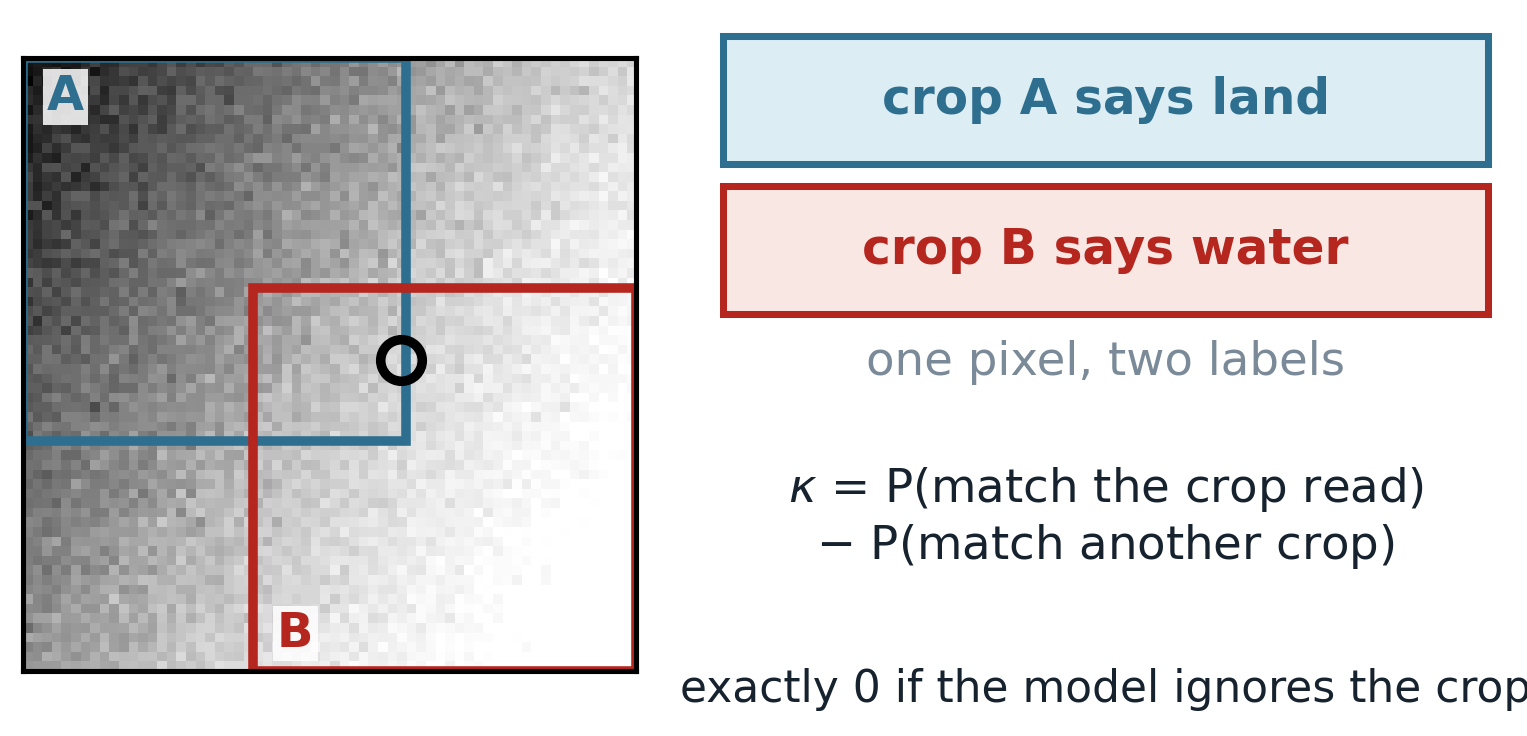
\includegraphics[width=\linewidth]{figures/fig0_mechanism.png}
\caption{The failure this paper measures. A labeller run inside each crop computes a
different threshold in each, here $-21.5$ and $-15.5$\,dB, so a pixel between them
comes out water in one window and land in the other.}
\label{fig:mechanism}
\end{figure}

Auto-labelling made large segmentation benchmarks possible. It also made some of
them circular, because the label can depend on which crop the model reads a pixel
in (\cref{fig:mechanism}). We are not aware of a diagnostic tailored to this
failure with an algebraically fixed reference value. Partial-input baselines answer the neighbouring
question~\cite{goyal2017making, jabri2016revisiting}, but diagnose a dataset by
training a second model and reading a gap whose null must be estimated. What is
needed here is an estimand whose value under crop-invariant predictions is known in
advance and whose label-only component can be computed on a benchmark one did not
build.

This paper supplies one, and applies it to two benchmarks. Foundation-model masks can
be used to construct remote-sensing segmentation labels~\cite{wang2023samrs}, and a
benchmark that adopts them per crop inherits the property it tests for.

\paragraph{Contributions.}
\begin{itemize}\itemsep2pt \parskip0pt \topsep2pt
\item A directional statistic, $\kap$, for how far a model's output tracks the
  crop it is reading, whose \emph{null} is exact rather than estimated: $\kap = 0$
  for any crop-invariant predictor on the fixed evaluated data, with no simulated
  null calibration (\cref{prop:null}). A matched contrast descriptively assesses
  whether excess alignment is associated with the training-label construction rather than an
  architecture-only floor (\cref{sec:floor}).
\item A calibration on Sen1Floods11 in which we rebuild the published labeller with
  a dial, and a within-chip threshold scramble that preserves each chip's threshold
  multiset while attenuating, but not eliminating, the threshold--input
  correspondence (\cref{sec:calib}).
\item A measurement on a 17-acquisition sea-ice benchmark we assembled from a
  published labeller, against a matched control trained on labels regenerated once
  per scene (\cref{sec:wild}).
\item A survey of labelling rules on public imagery with nothing trained, including
  the published labeller run per crop on chips it never saw, separating the rules
  that survive being applied per crop from those that do not
  (\cref{sec:survey}, \cref{sec:recovery}).
\item A single-file implementation with a self-test, and a protocol: label once per
  scene, split by acquisition, score each source pixel once (\cref{sec:recs}).
\end{itemize}

\paragraph{Terms.} A benchmark is \emph{crop-dependent} when one source pixel can
receive different labels depending on the crop it is read in. Computing labels from
the model's own input is not sufficient: a rule applied pointwise over a whole scene
reads those pixels and stays crop-invariant. \emph{Crop-label alignment} ($\kap$) is defined in
\Cref{sec:kappa}.

\section{Related work}
\label{sec:related}

Crop-dependent labelling sits between several literatures. The distinction this paper
turns on is the one between shortcut learning and label noise.

\paragraph{Shortcut learning.} Documented cases include
hospital-specific tokens in chest radiographs~\cite{zech2018variable}, background
rather than animal in wildlife recognition~\cite{beery2018terra}, and the general
account of shortcut learning as a property of gradient descent rather than of any
one dataset~\cite{geirhos2020shortcut, lapuschkin2019unmasking}. In each case the cue
was identified after a model had trained and generalised badly. Crop-label alignment
is a forward test with a value known under the null, so it names the cue in advance.

\paragraph{Annotation artefacts and partial-input baselines.} The closest analogues
are partial-input baselines. Hypothesis-only models on natural language inference
showed that labels were partly predictable from the annotation process, and that
leaderboard progress had been measuring that
predictability~\cite{gururangan2018annotation, poliak2018hypothesis}; vision does the
same with question-only baselines~\cite{goyal2017making, jabri2016revisiting}, whose
licensed inference has itself been questioned~\cite{feng2019misleading}. The
difference is that a crowdworker's habits cannot be recovered and an algorithmic
labeller can: we invert one to its constant in 17 of 17 folds and recover another's
threshold and kernel to within 0.25\,dB on 11 of 11 events, which lets us build the
artefact with a dial instead of only detecting it.

\paragraph{Relation to label noise.} The standard frame for imperfect
labels is noise, with a large literature on robust losses, noise-transition
estimation, and the observation that many test labels in standard benchmarks are
simply wrong~\cite{song2022learning, northcutt2021confident,
northcutt2021pervasive}. Crop-dependent error sits at one end of that literature
rather than outside it: input-independent noise supplies no stable input-predictive
signal, whereas instance-dependent noise can, and a crop-dependent label is the
limiting case, fixed by the crop the model is reading. A predictor can therefore
align with it and be rewarded under patch scoring where input-independent noise is
only penalised. The appropriate remedy is to generate labels outside the crop and
evaluate at source-pixel resolution.

\paragraph{Weak and programmatic supervision.} Labelling functions and
foundation-model pseudo-labels are two mechanisms that can produce crop-dependent
labels at scale~\cite{ratner2017snorkel,wang2023samrs}. What matters is what the labelling
function reads: a per-pixel rule survives being applied per crop, a rule with a
threshold estimated from the crop does not. Benchmarks shipping expert labels beside
algorithmic ones~\cite{aybar2022cloudsen12} would let $\kap$ and its association with
expert-label performance be
evaluated without constructing anything.

\paragraph{Overlapping windows and tiling artefacts.} Cross-window consistency has
been used as a training loss on overlapping predictions~\cite{dang2023crosswindow},
and remote-sensing work documents boundary errors from tiled inference and
stitching~\cite{huang2019tiling}. Recent reference-free seam metrics test whether
prediction gradients at tile boundaries differ from surrounding
content~\cite{carrara2026switi}. Those methods ask whether predictions agree across
windows or form visible seams. $P(\A)$ instead uses labels only, $\Omega$ uses
prediction variation only, and $\kap$ conditions on label disagreement and signs
that variation by which crop's label the prediction follows. Consequently seam or
consistency metrics can fire when labels are crop-invariant (where $\kap$ is
undefined), while $\kap=0$ can also hide cancelling signed effects. The diagnostic
is therefore narrower and complements overlap consistency.

\paragraph{Benchmark statistics.} A separate line argues that benchmark comparisons
are reported without the variance or the power to support them, and that seed and
data-order variation can exceed the differences
claimed~\cite{bouthillier2021accounting, reimers2017reporting, card2020little,
damour2022underspecification}. We therefore treat held-out folds as descriptive
evaluation units rather than independent replicates.

\paragraph{Spatial validation.} Splitting spatially autocorrelated data at random
inflates measured skill~\cite{roberts2017cross, ploton2020spatial,
karasiak2022spatial, kattenborn2022spatially}, and treating correlated observations
as independent replicates has a long history~\cite{hurlbert1984pseudoreplication};
the leakage taxonomy places this among failures that survive peer
review~\cite{kapoor2023leakage}. Our protocol repairs are the standard remedies
applied to a benchmark that used none; what we add is a diagnostic for the label
alignment that can remain after those choices.

\section{Crop-label alignment}
\label{sec:kappa}

\subsection{Definition}

A labeller produces, for each crop $c$ and each pixel $p$ inside it, a label
$L_c(p)$. When it reads only the pixels inside the crop, two crops covering the same
source pixel can assign it different labels. A predictor $f$ maps a pixel and the
crop it is read in to a class, written $f(p \mid c)$.

For a source pixel $p$, let $C(p)$ be the set of evaluated crops covering it and
supplying a valid label, and
$m(p) = |C(p)|$. The \emph{artefact set} is
\begin{equation}
\A = \{\, p : \exists\, c, c' \in C(p) \text{ with } L_c(p) \neq L_{c'}(p) \,\}.
\label{eq:aset}
\end{equation}
Off $\A$ the labeller is locally single-valued and there is nothing to detect. A
pixel covered by one crop can never enter $\A$, so $m(p) \geq 2$ throughout.

For $p \in \A$ and $c \in C(p)$, with $\ind{\cdot}$ the indicator, define
\begin{align}
\own(p,c) &= \ind{f(p \mid c) = L_c(p)}, \label{eq:own}\\
\oth(p,c) &= \frac{1}{m(p)-1} \sum_{c' \neq c} \ind{f(p \mid c) = L_{c'}(p)},
\label{eq:oth}
\end{align}
where here and below sums over $c$ or $c'$ run over $C(p)$. \Cref{eq:own} asks
whether the prediction matches the label of the crop being read, \cref{eq:oth} how
often it matches another covering crop's label. Averaging those differences over
\emph{source pixels},
\begin{equation}
\kap = \frac{1}{|\A|} \sum_{p \in \A} \frac{1}{m(p)}
       \sum_{c \in C(p)} \big[\, \own(p,c) - \oth(p,c) \,\big].
\label{eq:kappa}
\end{equation}
Each $p \in \A$ counts once. Averaging over $(p,c)$ instances instead gives
$\kapcr$, the \emph{crop-read} weighting, in which a pixel counts once per covering
crop; on $\A$, coverage runs from 2 to over 100, so the two differ. We report
\cref{eq:kappa} throughout and $\kapcr$ in the supplement. This statistic lies in
$[-1,1]$, is conditional on $p\in\A$, and is unrelated to Cohen's kappa despite the
shared symbol. We therefore report its disagreement prevalence
$P(\A)=|\A|/|\{p:m(p)>0\}|$ over evaluation-valid covered source pixels alongside
the primary benchmark results: $\kap$ describes alignment severity where labels
conflict, not how often conflict occurs.

\subsection{The null is exact}

\begin{proposition}
\label{prop:null}
Let $\A$ be non-empty and let $f$ be crop-invariant on $\A$, meaning
$f(p \mid c) = f(p)$ for every $p \in \A$ and every $c \in C(p)$. Then
$\kap = 0$ exactly.
\end{proposition}

\begin{proof}
Fix $p \in \A$, write $m = m(p)$ and $y = f(p)$, which by hypothesis does not depend
on the crop. For each class $k$ let $n_k = |\{ c \in C(p) : L_c(p) = k \}|$, so that
$\sum_k n_k = m$. Summing \cref{eq:own} over the crops covering $p$,
\begin{equation}
\sum_{c} \own(p,c) = \sum_{c} \ind{y = L_c(p)} = n_y .
\label{eq:sumown}
\end{equation}
Summing \cref{eq:oth} and exchanging the order of summation,
\begin{align}
\sum_{c} \oth(p,c)
  &= \frac{1}{m-1} \sum_{c} \sum_{c' \neq c} \ind{y = L_{c'}(p)} \nonumber \\
  &= \frac{1}{m-1} \sum_{c'} \ind{y = L_{c'}(p)} \cdot (m-1) \nonumber \\
  &= n_y ,
\label{eq:sumoth}
\end{align}
because each $c'$ is counted once for every $c$ other than itself, that is $m-1$
times, and the normaliser cancels it.

So \cref{eq:sumown} and \cref{eq:sumoth} agree at every $p \in \A$, and therefore
\begin{equation}
\sum_{c \in C(p)} \big[ \own(p,c) - \oth(p,c) \big] = n_y - n_y = 0
\quad \text{for every } p \in \A .
\label{eq:innerzero}
\end{equation}
\Cref{eq:kappa} is a weighted sum of that inner quantity, so it is $0$; and because
\cref{eq:innerzero} holds pixel by pixel, \emph{any} weighting over $p$ gives $0$,
including $\kapcr$.
\end{proof}

Nothing in the argument uses the number of classes, the label distribution, the
coverage $m(p)$, or any property of the imagery; it needs only that $\A$ is
non-empty, since $\kap$ averages over the source pixels in it. For fixed evaluated
predictions, zero is an algebraic identity rather than a null distribution that must
be simulated or estimated. This says nothing by itself about population uncertainty
across scenes.

\begin{corollary}
\label{cor:dep}
$\kap \neq 0$ certifies that $f$ is crop-dependent on $\A$.
\end{corollary}

The converse does not hold: $\kap$ sums signed contributions, so alignment and
anti-alignment may cancel, and $\kap = 0$ does not certify crop-invariance.
Attributing a positive $\kap$ specifically to the training-label construction needs
the matched control of \Cref{sec:floor}. So the exact zero is an algebraic identity
and a check on the code, a nonzero $\kap$ is directional, and our primary comparative
conclusions use the treated arm minus its matched control.

\subsection{Why the measured control is not zero}
\label{sec:floor}

A convolutional network reading crops is not a crop-invariant predictor. Zero
padding at the crop border, receptive fields truncated at the window edge, and any
normalisation computed over the crop all make $f(p \mid c)$ depend on $c$ near
boundaries. This is not our observation: convolutional layers are known to read
absolute position from padding~\cite{kayhan2020translation, islam2020position} and to
develop border artefacts because of it~\cite{alsallakh2021mind}. We measure the
consequence directly as $\Omega$, the probability that two crops covering the
same pixel predict differently. Writing $P$ for the pixels with $m(p) \ge 2$,
\begin{equation}
\Omega = \frac{\sum_{p \in P} \sum_{c \neq c' \in C(p)}
        \mathbf{1}[\, f(p \mid c) \neq f(p \mid c') \,]}
       {\sum_{p \in P} m(p)\big(m(p) - 1\big)}.
\label{eq:omega}
\end{equation}
The inner sum is over ordered crop pairs $(c,c')$; the denominator therefore has
$m(p)(m(p)-1)$ terms for pixel $p$.
It sums over every covered pixel rather than over $\A$, since it is a property of
the model and is defined where the labels agree, and weights crop pairs uniformly
rather than source pixels. It is shift consistency~\cite{zhang2019shiftinvariant} on
overlapping windows, and reads $0.031$ for optical-only sea-ice models on repaired labels and
$0.0108$ for flood models on the published ones.

How far this lifts $\kap$ off zero depends on how crop-invariant the labels really
are, and the two benchmarks answer differently. On flood labels regenerated from the
published per-event threshold, which are crop-invariant exactly, a trained network
reads $\kap = -0.0008$, empirically near the theoretical zero. On sea ice the
optical-only repaired control reads $+0.0097$. That is consistent with the labels still
inheriting a per-scene normalisation a $128 \times 128$ window can partly
recover, though we have not isolated that from the other crop effects above.

So the floor is not convolution alone: $\Omega$ is positive
on both benchmarks while $\kap$ reads $-0.0008$ on one and $+0.0097$ on the other,
which a resolution floor could not do. Crop-invariant training labels do not on their
own hold $\kap$ at zero, and \cref{prop:null} does not say they do: it constrains
predictors, not labels. The floor is an interaction of labels, model, crop grid and
imagery, which is why every attribution claim below uses a contrast between a
crop-dependent arm and its matched control on the same grid; raw values are shown to
expose the floor.

\section{Verifying the estimator, and bounding its scope}
\label{sec:verify}

\subsection{A case with a known answer}

\cref{prop:null} supplies something rarer than a null: an input whose correct output
is known before looking, which gives a direct test of the code. A
per-pixel threshold on chip-level smoothed VH reads one pixel value and cannot see a
window, so it is exactly crop-invariant. The estimator
must return zero.

Measured on four held-out flood events, on the same artefact set as every other arm
and between 9.5 and 41 million deterministic crop-pixel reads per event, $|\kap|$ stays below
$1.4 \times 10^{-15}$ and $\Omega$ is exactly zero in all four. What remains is accumulated
floating-point rounding.

An error in the $(m-1)$ normaliser, the own-versus-other bookkeeping or the
artefact-set mask surfaces here as a nonzero number. Not every error does: the
weighting and lifecycle faults can pass this arm, so the released suite tests
them separately with a nonuniform-coverage exact-value case and lifecycle
regressions.

\subsection{Which labelling rules can produce the artefact}
\label{sec:survey}

The artefact set depends only on a labelling rule and a crop grid, not on any model,
so it can be computed on imagery we did not assemble and without training anything.
We ran six rules used in SAR water mapping over 445 of the 446 released Sen1Floods11
chips, one having no valid backscatter, applying each rule separately inside every
crop of a $128 \times 128$ stride-32 grid and measuring $P(\A)$: the share of
covered source pixels whose valid covering-crop labels disagree.

\begin{table}[tb]
\centering
\scriptsize
\setlength{\tabcolsep}{1.4pt}
\begin{tabular}{lccc}
\toprule
labelling rule & fit inside crop? & mean $P(\A)$ & max \\
\midrule
fixed global constant        & no  & $0.00\%$  & $0.00\%$ \\
Otsu, computed per scene     & no  & $0.00\%$  & $0.00\%$ \\
Otsu, computed per crop      & yes & $17.58\%$ & $40.90\%$ \\
$k$-means, per crop          & yes & $17.65\%$ & $40.70\%$ \\
45th percentile, per crop    & yes & $16.02\%$ & $32.49\%$ \\
min-max per crop, then fixed & yes & $12.54\%$ & $54.82\%$ \\
\bottomrule
\end{tabular}
\caption{Artefact set produced by six labelling rules on 445 public Sen1Floods11
chips, 169 crops each. Mean and maximum are over chips after excluding the one chip
with no valid backscatter. No model is involved. A rule with $P(\A) = 0$ leaves
$\kap$ undefined rather than zero: there is nothing to average over.}
\label{tab:survey}
\end{table}

The $17.58\%$ here and the $24.71\%$ calibration reference in
\cref{tab:calib} are not interchangeable prevalence estimates. This survey fits
Otsu to raw VH, skips failed crops and averages chip-level fractions over 445 chips.
The calibration uses a $9\times9$-smoothed field with finite fallbacks on a common
440-chip set, pools source pixels within each event, then averages the eleven event
fractions.

\paragraph{Two further surveys.} The four crop-adaptive rules in \cref{tab:survey}
fit a threshold or normalisation inside each crop.
Labels built from foundation-model masks do the opposite, fixing the threshold and
recomputing the \emph{segmentation}: SAM run inside each crop of 37 chips reads nonzero
on all 37, median $1.13\%$ and mean $8.80\%$, up to $43.64\%$, where the same regions
computed once per scene read exactly $0.00\%$. This is an out-of-distribution stress
test of natural-image SAM on duplicated SAR channels; we do not interpret it as a
prevalence estimate. A
third moves to 342 public CloudSEN12+ patches~\cite{aybar2024cloudsen12plus} and cloud
masking. On a $128\times128$, stride-32 grid (144 crops per $509\times509$ patch), the
same clear-sky percentile fitted per crop instead of per scene reads $26.57\%$ and
loses $0.079$ of balanced accuracy against that dataset's expert masks. Accuracy is
reported there because $P(\A)$ counts whether covering crops agree, not whether they
are right, so a labeller calling everything cloud would score a perfect zero.

The zeros are exact, on every chip and in all three surveys. Otsu is the same
estimator in rows two and three of \cref{tab:survey} and differs only in the pixels it
is computed over. Applying a labeller per crop is therefore not what creates the
hazard. Context-sensitive computation inside the crop is, whether a threshold, a
normalisation, a background estimate or the segmentation itself, and that is a
narrower and more actionable thing to check for.

\subsection{\texorpdfstring{$\kap$}{kappa} is relative to the crop grid}
\label{sec:grid}

How densely crops are sampled is a choice we made, so we thinned the evaluation grid
from stride 32 to stride 64 on identical models and labels, recomputing nothing. The
contrast rises from $+0.2666$ to $+0.4587$, a factor of $1.72$, while the two
geometries still order the eleven events at Spearman $r = +0.918$: the magnitude moves
and the ranking survives. The supplement gives the mechanism.

The encoder moves it little. Both ends rerun with a transformer encoder and with a
second convolutional one stay positive in 11 of 11 events, at $+0.2966$ and $+0.2943$
against $+0.2666$ for the U-Net on seed 42, with trained-control values empirically
near zero in all three. The sign and rough size survive; both replacements read about $10\%$
above the U-Net. We report this gap without an equivalence test. The trained controls are
empirically near zero; only the crop-invariant predictor in \cref{prop:null} has an
exactly zero theoretical value.

So $\kap$ compares arms sharing one crop geometry: its magnitude does not travel
between papers that tile differently, and without a crop size and stride it cannot
be read.

\section{Experimental setup}
\label{sec:setup}

\begin{figure*}[t]
\centering
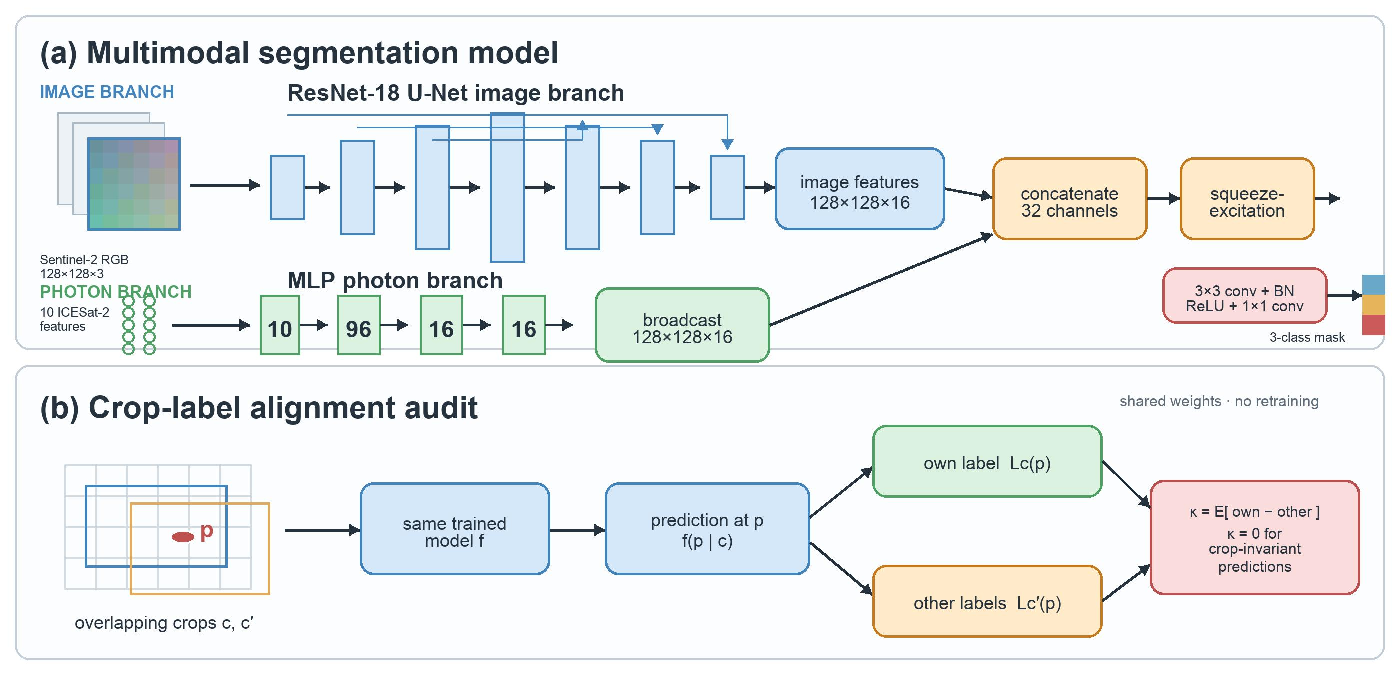
\includegraphics[width=0.72\textwidth]{figures/crop_alignment_architecture.pdf}
\caption{Model and audit schematic. The sea-ice model uses an ImageNet-initialized
ResNet-18 U-Net image branch and, in photon-enabled runs, an MLP branch for ICESat-2
features. The audit keeps weights fixed and compares agreement with the current
crop's label against other crops' labels for the same source pixel.}
\label{fig:architecture}
\end{figure*}

The supplement gives the full configuration. The sea-ice benchmark has 169{,}051
patches over 39 tiles and 17 acquisitions; the flood benchmark has 446 chips over 11
events, and the crop sweep draws 24 crops per chip per epoch from a $13 \times 13$
grid, evaluating $\kap$ on all 169 positions. The sea-ice model carries a second
branch that encodes ten co-registered ICESat-2 photon
features~\cite{neumann2019atlas} (\cref{fig:architecture}). The primary $\kap$ arm, at seed 42, disables that
branch and is optical-only. A seed-7 photon-enabled run is reported separately as an
input-mode sensitivity check, not averaged as a repeat seed.

Splits are leave-one-acquisition-out and leave-one-event-out, since that is the unit
sharing a labeller constant, and model selection never sees the held-out unit.
For crop-label alignment, both scorers retain every crop-read prediction and use
the source-pixel weighting, so each source pixel in the artefact set has equal
weight. Only the flood expert-label analysis mosaics hard predictions by majority
vote before scoring each source pixel once.

Training used two RTX A6000 cards capped at 300\,W; flood crop runs take about four
minutes each. Full optimisation settings are in the supplement.

\section{Calibrating the diagnostic}
\label{sec:calib}

The sea-ice benchmark cannot establish sensitivity, because the crop-dependence of
that pipeline is the unknown being estimated. So we built a labeller with a dial. Sen1Floods11~\cite{bonafilia2020sen1floods11}
ships an Otsu-on-VH~\cite{otsu1979threshold} label set with one published threshold
per flood event, whose preprocessing we recover in \Cref{sec:recovery}. Holding that
smoothing fixed and recomputing only the threshold inside each crop reproduces the
sea-ice mechanism with one scalar per crop as the entire source of crop-dependence:
\begin{equation}
\tau_c(\alpha) = (1-\alpha)\,\tau_{\text{event}} + \alpha\,\tau_{\text{crop}} .
\label{eq:dial}
\end{equation}
At $\alpha = 0$ the labels are the published ones, crop-invariant by construction. At
$\alpha = 1$, Otsu returns a crop threshold at 72{,}029 of 75{,}374 positions
(95.56\%); 2{,}331 (3.09\%) use a finite chip fallback, while 1{,}014 positions in
six chips (1.35\%) remain unusable and those chips are excluded from every arm. The within-chip range averages
6.13\,dB. The endpoint also shifts the mean threshold from $-21.798$ to
$-17.796$\,dB. The dial controls crop fitting but does not isolate
crop-dependence.

The artefact set \emph{and the labels it is scored against} are both fixed at
$\alpha = 1$: write $\kap_{L^\star\!,\A^\star}(f_\alpha)$ for the model trained at
$\alpha$ read against that fixed reference. Rebuilding either per arm would empty
$\A$ at $\alpha = 0$, leaving the control with no pixels to be null on. So $\kap$
there is an empirical near-zero from a model that never learned the artefact; it is
separate from the proposition's identity. Sea ice works the same way.

\begin{figure}[tb]
\centering
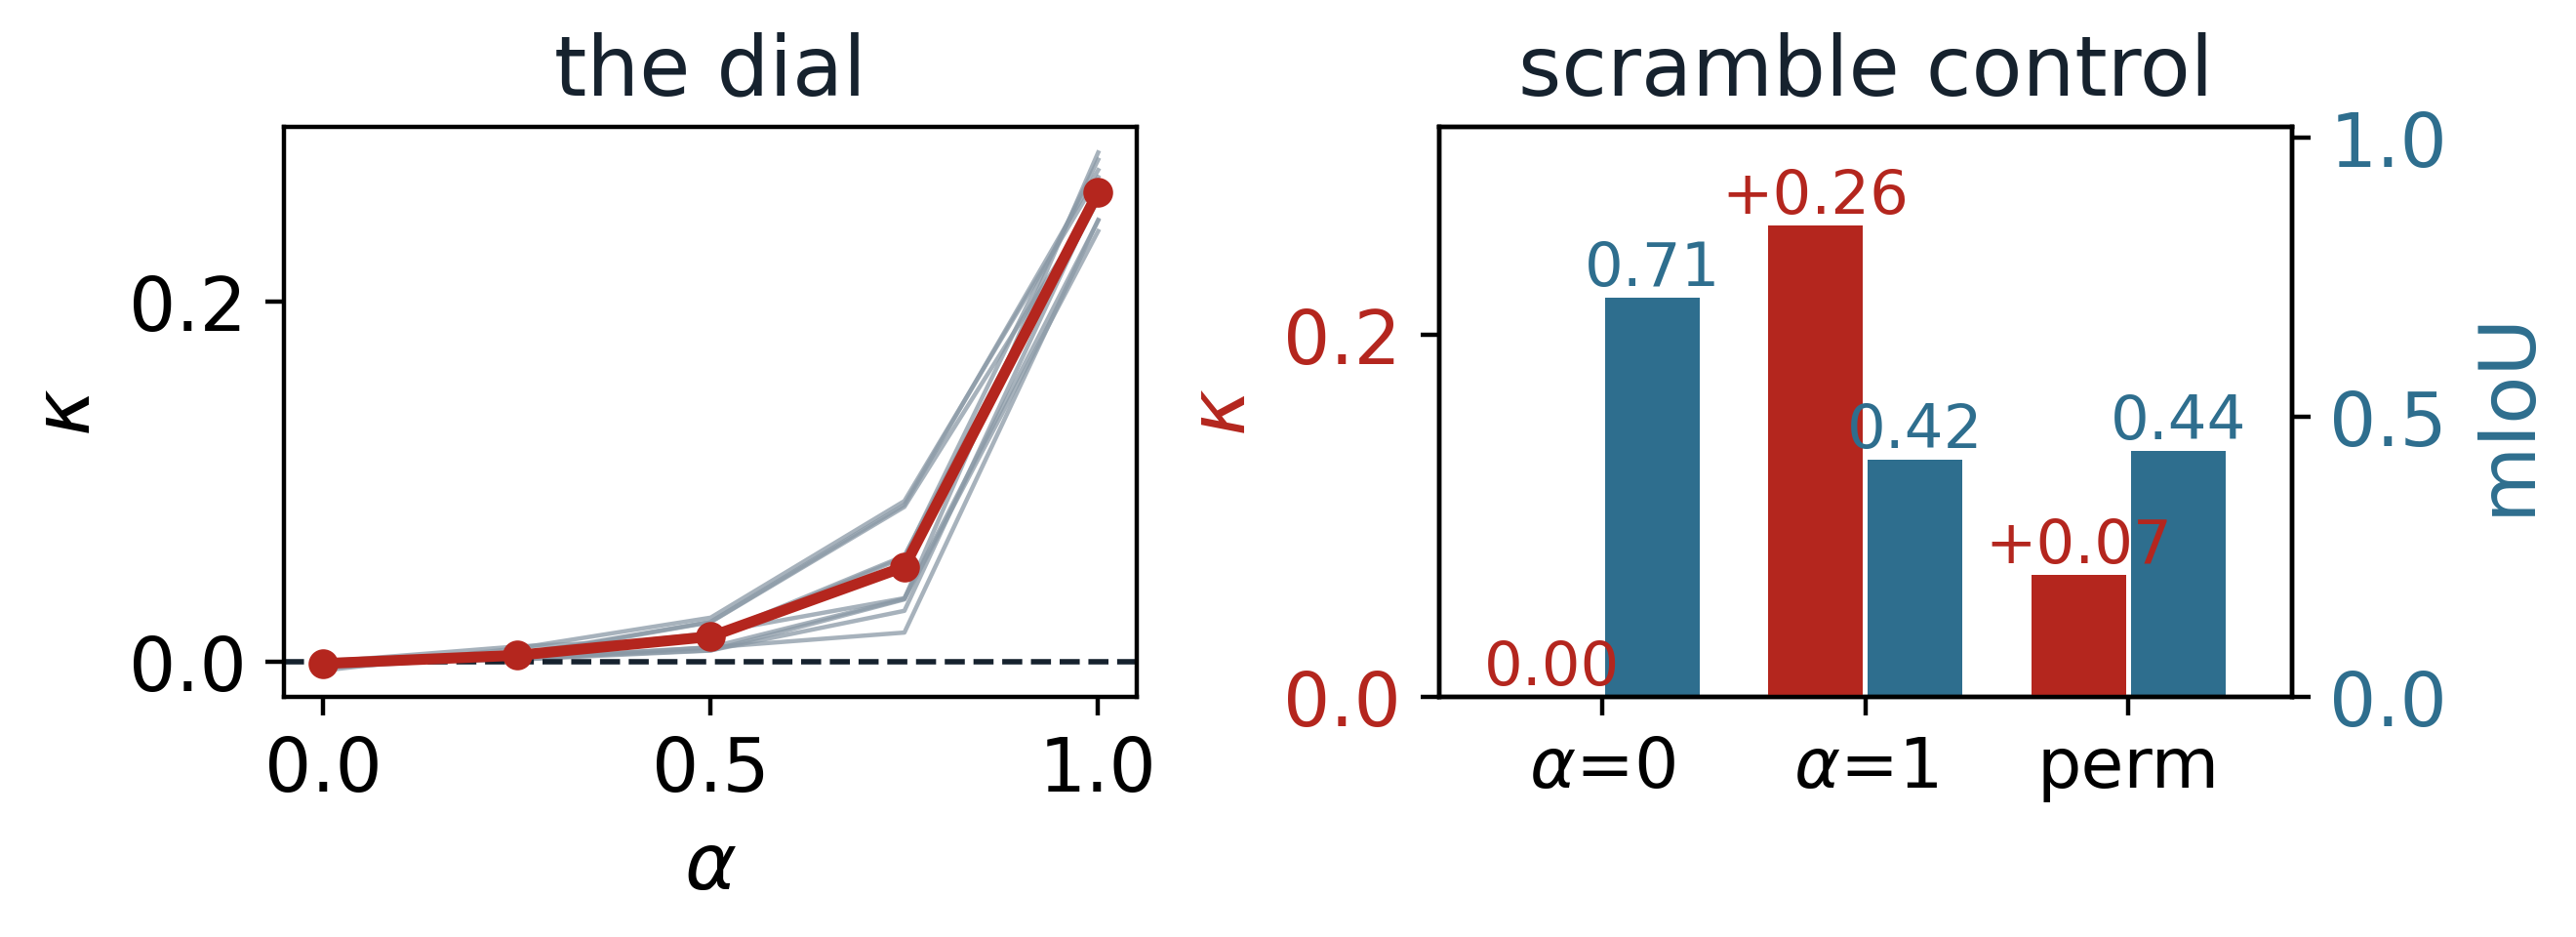
\includegraphics[width=\linewidth]{figures/fig4_calibration.png}
\caption{Left: $\kap$ against the dial of \cref{eq:dial}, grey lines held-out events
and red the mean; the dashed line marks the algebraic zero. $\alpha = 0$ is the
published threshold, while $\alpha = 1$ is
predominantly crop-fitted (95.56\% direct fits; the remainder is accounted for in text).
Right: those arms and \emph{scramble}, one random reassignment of threshold positions
within each chip; $\kap$ red on the left axis, mIoU against expert labels blue on the
right. It preserves the threshold multiset but does not eliminate spatial dependence.}
\label{fig:calib}
\end{figure}

\begin{table}[tb]
\centering
\scriptsize
\setlength{\tabcolsep}{1.3pt}
\resizebox{\linewidth}{!}{%
\begin{tabular}{@{}lccccc|cc@{}}
\toprule
 & \multicolumn{5}{c|}{dial, $\alpha$} & \multicolumn{2}{c}{controls} \\
 & 0.00 & 0.25 & 0.50 & 0.75 & 1.00 & scramble & offset \\
\midrule
$\kap$   & $-0.0008$ & $+0.0037$ & $+0.0141$ & $+0.0528$ & $\mathbf{+0.2605}$ & $+0.0672$ & $-0.0003$ \\
$\Omega$ & 0.0108 & 0.0132 & 0.0211 & 0.0454 & 0.1119 & 0.0933 & 0.0121 \\
mIoU     & 0.714 & 0.696 & 0.673 & 0.604 & $\mathbf{0.423}$ & 0.440 & 0.715 \\
\bottomrule
\end{tabular}
}
\caption{Crop-label alignment, model crop-dependence and accuracy against expert
labels, averaged descriptively over the eleven held-out events. Every $\kap$ uses the
same $\alpha=1$ reference set, with $P(\A^\star)=24.71\%$. \emph{Scramble} randomly
reassigns thresholds within each chip; \emph{offset} is constant within a chip and
varies only between chips.}
\label{tab:calib}
\end{table}

The three diagnostics in \cref{tab:calib} answer different questions. The fixed
$P(\A^\star)$ is a label-only prevalence and cannot rank these models; $\Omega$ is
unsigned prediction inconsistency and remains positive for both near-zero controls.
Only $\kap$ records the signed association between a prediction and the label of the
particular crop being read.

\cref{tab:calib} and \cref{fig:calib} give the result. The contrast between the ends
is $+0.2613$ (sd $0.0149$), positive in 11 of 11 events after averaging seeds within
event, and per-event rank
correlation with $\alpha$ is perfect in all eleven. At
$\alpha = 0$, where the labels are the published ones and crop-invariant exactly,
$\kap$ reads $-0.0008$.

\paragraph{What changes across the dial.} A threshold recomputed on a water-poor
$128 \times 128$ window is not only crop-dependent, it is worse: accuracy against
expert labels falls by $0.29$ mIoU across the dial. None of the dial values isolates
crop adaptation from the accompanying changes in threshold and label quality. The
scramble arm is a sensitivity check and does not isolate causality. Within
each chip it preserves the exact threshold multiset, but the unconstrained random
permutation leaves 461 of 75{,}374 assignments (0.61\%) fixed and pairs 21.78\% of
recipients with a geometrically overlapping donor crop; all donors also share the
same chip. These geometry counts describe the full serialized mapping, including
the six chip rows excluded from training and scoring. In this one reassignment, model performance retained 94\% of the endpoint
mIoU difference ($-0.2736$ versus $-0.2905$), while $\kap$ fell from $+0.2605$ to
$+0.0672$, leaving 26\% of the endpoint excess. That residual cannot be partitioned
among generic crop-varying labels, overlap, and same-chip predictability. The offset
arm, varying the threshold once per chip at the same spread, yields $-0.0003$.

\paragraph{Dependence of fold summaries.} The eleven events are distinct, but
the eleven models are leave-one-event-out folds sharing nearly all of their
training data, so a $t$ or a sign test over them assumes an independence the
design does not provide, exactly as on sea ice. \Cref{tab:seeds} offers
a training-seed sensitivity check instead: the aggregate contrasts vary by less
than $0.011$ across three seeds. This shows stability on the same folds. It does not
provide independent replication or reassignment uncertainty because all three seeds
use the same scramble; Table~\ref{tab:seeds} lists those seed-wise contrasts.

\begin{table}[tb]
\centering
\footnotesize
\setlength{\tabcolsep}{4pt}
\begin{tabular}{lccc}
\toprule
contrast & seed 7 & seed 42 & seed 123 \\
\midrule
$\alpha{=}1$ against $\alpha{=}0$ & $+0.2601$ & $+0.2666$ & $+0.2573$ \\
$\alpha{=}1$ against scramble & $+0.1992$ & $+0.1919$ & $+0.1888$ \\
\bottomrule
\end{tabular}
\caption{Training-seed sensitivity of the dial. Each cell is the mean over the same
eleven held-out events, so the exact ranges across seeds are $0.0093$ and $0.0104$ against
effects of $+0.26$ and $+0.19$.}
\label{tab:seeds}
\end{table}

\paragraph{Scope.} Sen1Floods11 as published computes one threshold per event, so the
crop-dependent artefact is not present in that benchmark. The imagery and the labeller
are real and the crop-dependence is ours. This experiment calibrates the diagnostic;
it does not establish a second real-world occurrence, and nothing here bears on that
dataset's published labels.

\section{Association with expert-label performance}
\label{sec:cost}

The models of \Cref{sec:calib} were trained, validated and tested inside their own
algorithmic label field. We additionally score each model against the expert labels
that Sen1Floods11 ships, without new training. A mosaic majority vote gives one
decision per source pixel before comparison; patch scoring would count each pixel
about sixteen times and reward the crop-specific target repeatedly.

Expert-label mIoU decreases monotonically from $0.714$ to $0.423$ across the
constructed dial, an endpoint difference of $-0.2905$ (descriptive sd $0.0918$),
with the same direction in all eleven held-out events. This is the combined result of
replacing published event thresholds with predominantly per-crop Otsu labels. It is
not the causal cost of crop-dependence: the endpoint also moves the mean threshold by
4.00\,dB and changes class balance, boundaries and raw label quality.

After subtracting each event's mean, $\kap$ and expert-label mIoU have descriptive
$r=-0.928$ and a slope of $-1.05$ mIoU per unit $\kap$ across the five dial levels.
Because $\alpha$ jointly drives both axes, this is a joint dose response, not evidence
that $\kap$ predicts damage beyond the dial. Fixed-$\alpha$ correlations do not give
that stronger result: their average is $-0.196$, with signs ranging from $+0.774$ at
$\alpha=0$ to $-0.087$ at $\alpha=1$.

The within-chip scramble gives a limited sensitivity check. In its one threshold
reassignment, 94\% of the endpoint mIoU difference remained while the alignment fell
to 26\%. Since the mapping allows fixed points, overlapping donor crops and same-chip
spatial dependence, we do not interpret that contrast as isolating a mechanism.

\section{Applying and reconstructing two published labellers}
\label{sec:wild}

\subsection{What we recovered, and on whose data}
\label{sec:recovery}

\paragraph{Provenance, and which step is the culprit.} We are explicit about what is
ours, because it bears on how far this generalises. The colour labeller is
published~\cite{iqrah2023polar,iqrah2024parallel}, and so is the practice of cutting
Sentinel-2 patches on ICESat-2 track points one pixel apart, which produces densely
overlapping windows~\cite{lechamo2025multimodal}. The 17-acquisition assembly is ours:
our co-location, our $128 \times 128$ geometry, our class-stratified subsample.

The published colour thresholds are \emph{fixed constants}, and the released code
applies them after splitting a scene into patches. What makes our label set
crop-dependent is one stage earlier, a cloud and shadow removal that fits three
quantities to the array it is handed: an Otsu threshold, a median-blur background
estimate, and two min-max normalisations. Labelling per crop is not the hazard, since
a fixed rule survives it. Context-sensitive computation inside the crop is what
creates it, though not every
fitted step contributes, and the experiments below identify which ones do.

\paragraph{External imagery.} We tested the released labeller on the 446
public Sen1Floods11 optical chips on the same stride-32 grid. Nothing is trained and
input scaling is one global constant, so any $P(\A) > 0$ certifies crop dependence
of the rule under this fixed preparation; the class names do not describe flood scenes and need not,
since $P(\A)$ measures agreement among crops without judging correctness. Two arms
serve as code controls: stage 1 alone, and the
stage with every fitted quantity taken from the scene, are compositions of per-pixel
functions and must read zero. Both do, exactly. Fitted per crop as released the stage
reads $37.04\%$. Repairing its background and Otsu threshold cuts that by $88\%$ to
$4.50\%$, but the worst chip falls only from $57.90\%$ to $40.07\%$, and the two
normalisations, inert while the other quantities are fitted per crop, carry what is
left: a partial repair is not a repair. The supplement ablates each step and varies
the one preparation constant we chose, which the residual is sensitive to and the
$37.04\%$ is not.

\paragraph{Sea ice.} OpenCV hue ends at 179, below the published upper threshold of
185, so only the value channel acts; a grid search recovers the water constant in all
17 folds. Crop-dependence enters through the cloud and shadow stage, run here on
$128 \times 128$ patches with a 155-pixel median kernel. Scene-wide regeneration
raises crop unanimity from $0.9678$ to $1.0000$ in every fold.

\paragraph{Floods.} Sen1Floods11 ships an expert label and an Otsu label for the
same 446 chips, and unlike the sea-ice case it publishes the constant, so the
recovery can be checked from outside. Thresholding the raw band leaves a bias of one
sign on all eleven events, a systematic signature, and the supplement
sweeps the smoothing radius to find it: a $9 \times 9$ focal mean before thresholding
lands all eleven within $0.25$\,dB at $99.08\%$ agreement. The constant moves 5.57\,dB
across events, so no global threshold can express it and a model seeing the whole
chip can infer which event it is in and adapt.

\subsection{Crop-label alignment on the sea-ice benchmark}

Sea-ice crops overlap about 33 times, so a source pixel is seen inside many crops,
and under the per-crop scheme those crops can disagree. Across all 17 folds, with
$\A$ averaging 13.22\% of covered pixels and 23.9M deterministic crop-pixel reads per fold, the model
trained on crop-noisy labels in the optical-only primary arm (seed 42) reads
$\kap = +0.1518$. Its matched control, trained on repaired labels and evaluated on
identical pixels, reads $+0.0097$. The mean paired difference is
$\mathbf{+0.1421}$, and it is positive on each of the 17 dependent evaluation
folds. A photon-enabled sensitivity at seed 7 reads a $+0.1454$ contrast, also
positive in 17 of 17 folds. Because input mode and initialization change together,
this serves only as a robustness check because it cannot estimate seed replication.
\Cref{fig:wild} gives
the optical-only primary per-fold results against their controls.

We report that descriptively and attach no test to it. These 17 folds are overpasses
of 39 tiles across 25 days sharing tiles, geography and almost all of their training
data, so a $t$ or an interval over them would assume an independence the design does
not provide. We therefore omit inferential summaries over folds.

\begin{figure}[tb]
\centering

\includegraphics[width=\linewidth]{figures/fig2_crop_alignment.png}
\caption{Optical-only primary crop-label alignment (seed 42) per held-out
acquisition. Red is the model trained on crop-noisy labels, blue its matched control
trained on labels regenerated once per scene. Zero is the theoretical identity for
crop-invariant predictors; the trained control is empirical and need not equal it.}
\label{fig:wild}
\end{figure}

We do not express this as a fraction of the calibrated contrast of \Cref{sec:calib}:
the two used different crop grids, and \Cref{sec:grid} shows a grid change moves the
contrast by more than any such ratio would report. Two consistency checks follow. On
the repaired label set $\A$ is empty, since crop unanimity of $1.0000$ means every
covering crop agrees. And $\Omega$ is exactly zero for the two-parameter threshold,
whose value channel is a per-pixel function of per-fold constants.

\section{Discussion}
\label{sec:recs}

The practical fix is simple: fit contextual quantities on support containing all
evaluation crops that cover a source pixel, persist one label per source pixel,
split by the labeller's dependence unit, score each source pixel once, and report a
context-free baseline. Reviewers should ask for $\kap$ on a stated crop grid with a
matched control. The algebraic zero checks the diagnostic; the control separates
excess alignment from an architecture floor.

The limits are part of the claim. $\kap$ is grid-relative: changing the crop grid
changes the disagreement set and can move the magnitude without retraining. The
scramble arm preserves each chip's threshold multiset, but does not fully break
threshold--image coupling. Folds share geography, tiles and training data, so we
report signs and matched contrasts descriptively rather than fold-level inference.
The diagnostic sees only locations where overlapping crop labels disagree; it misses
crop-invariant pseudo-label shortcuts, calibration failures and unrelated shortcuts,
and opposite signed regions can cancel. Sea ice has no human reference labels, so it
shows excess alignment with crop-dependent labels, not expert-label harm.


\iftoggle{wacvfinal}{\paragraph{Code and data.}
The public repository is available at \url{\publicCodeURL}.}{}

% lineno can place two independent numbers into the bibliography gutter when a
% reference wraps across columns.  Keep review lines on the entire paper body, but
% disable them for references so the rendered entries remain legible.
\nolinenumbers
{
    \small
    \bibliographystyle{ieeenat_fullname}
    \bibliography{main}
}

\end{document}
